\documentclass[12pt, openany]{report}
\usepackage[T1]{fontenc}
\usepackage[english]{babel}
\usepackage{csquotes}
\usepackage[margin=1in]{geometry}
\usepackage{setspace}
\usepackage{microtype}
\usepackage{amsmath, amssymb, amsthm}
\usepackage{graphicx}
\usepackage{booktabs}
\usepackage[style=authoryear]{biblatex}
\addbibresource{references.bib}
\usepackage[colorlinks=true, allcolors=blue]{hyperref}

\onehalfspacing

\begin{document}

\pagenumbering{alph}
\begin{titlepage}
  \centering
  {\large\scshape Institution \par}
  {\large Department \par}
  \vspace{3cm}
  {\huge\bfseries {{TITLE}} \par}
  \vspace{2cm}
  {\Large {{AUTHOR}} \par}
  \vspace{2cm}
  A thesis submitted in partial fulfillment of the requirements \par
  for the degree of Master of Science \par
  \vspace{1cm}
  Supervised by Supervisor's name \par
  \vfill
  {\large \today \par}
\end{titlepage}

\pagenumbering{roman}
\chapter*{Acknowledgments}
\addcontentsline{toc}{chapter}{Acknowledgments}

The acknowledgments name the people and organizations that supported this
work.

\chapter*{Abstract}
\addcontentsline{toc}{chapter}{Abstract}

The abstract sets out in one page the problem, the method, the results and
the conclusions of the thesis.

\tableofcontents
\listoffigures
\listoftables

\cleardoublepage
\pagenumbering{arabic}
% Each chapter is in its own file of the chapters folder.
\chapter{Introduction}
\label{chap:introduction}

The introduction sets out the context, the problem and the objectives of the
thesis, then outlines it: Chapter~\ref{chap:background} reviews existing
work, Chapter~\ref{chap:method} describes the method and
Chapter~\ref{chap:conclusion} concludes.

Each chapter is a file of the \texttt{chapters} folder, included in
\texttt{main.tex} by an \verb|\include| command.

\chapter{Literature review}
\label{chap:background}

This chapter places the thesis among existing work. The references are in
\texttt{references.bib}: \textcite{knuth1984} describes \TeX{} and
\textcite{lamport1994} presents \LaTeX{}. References can also be cited in
parentheses \parencite{mittelbach2023}.

\chapter{Method and results}
\label{chap:method}

\section{Method}

The method relies on the model
\begin{equation}
  \label{eq:model}
  \frac{\mathrm{d}x}{\mathrm{d}t} = -\lambda x, \qquad x(0) = x_0,
\end{equation}
whose solution is $x(t) = x_0 e^{-\lambda t}$.

\section{Results}

Figure~\ref{fig:results} and Table~\ref{tab:results} present the results
obtained with model~\eqref{eq:model}.

\begin{figure}[htbp]
  \centering
  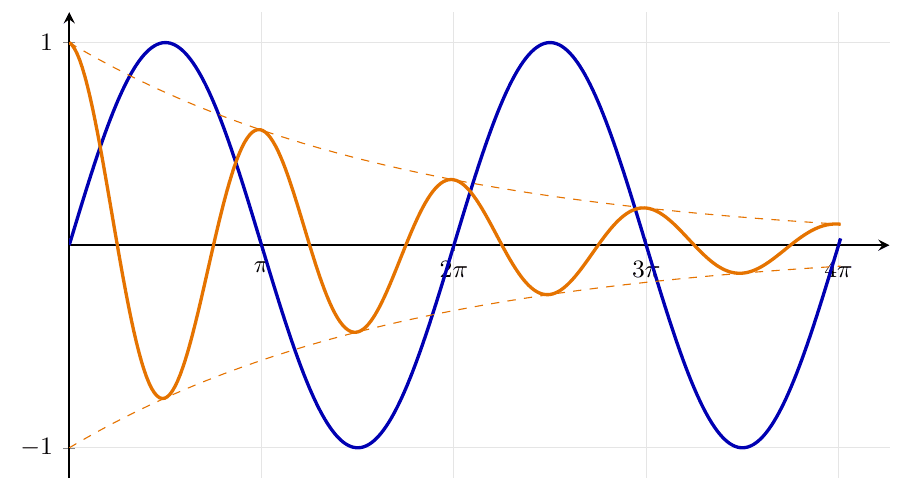
\includegraphics[width=0.75\linewidth]{images/curves.png}
  \caption{An image of the project: replace it with your results.}
  \label{fig:results}
\end{figure}

\begin{table}[htbp]
  \centering
  \caption{Estimated values of the parameter $\lambda$.}
  \label{tab:results}
  \begin{tabular}{lrr}
    \toprule
    Trial & $\lambda$ & Relative error (\%) \\
    \midrule
    1 & 0.182 & 1.1 \\
    2 & 0.179 & 0.6 \\
    3 & 0.185 & 2.8 \\
    \bottomrule
  \end{tabular}
\end{table}

\chapter{Conclusion}
\label{chap:conclusion}

The conclusion sums up the contributions of the thesis, discusses their
limits and suggests further research.


\printbibliography[heading=bibintoc]

\appendix
\chapter{Additional data}
\label{chap:appendix}

The appendices gather long proofs, data and code.


\end{document}
